\section{Spatiotemporal Pauli processes}\label{sec:spp}
We now introduce \emph{spatiotemporal Pauli processes} (SPPs), the effective stochastic processes induced by applying the \emph{multi-time Pauli twirl} to a quantum process tensor. The twirl maps an arbitrary (possibly non-Markovian) process to a joint distribution over spatiotemporal Pauli trajectories, eliminating genuinely quantum temporal correlations while retaining arbitrary classical correlations. Crucially, in a tensor-network representation this map is implemented by fixed local contractions on the physical legs at each time step, leaving the virtual (environment) bonds unchanged. This yields an explicit classical tensor network---an MPS in 1D and a PEPS in 2D---encoding the trajectory weights (and hence probabilities). As a direct consequence, the temporal bond dimensions of the resulting SPP tensor networks are bounded by the corresponding process tensor bonds, and in particular by the environment Liouville dimension \(d_E^2\) for finite environments. These results justify SPPs as a natural tensor-network-compatible description of correlated circuit-level Pauli noise, and provide the technical foundation for the explicit noise models and QEC studies developed in later sections.

\subsection{Multi-time Pauli twirling and SPPs}
We begin by extending the standard Pauli twirling operation for quantum channels to multi-time processes.

Let \(\mathbb{P}^{(n)}\) denote the \(n\)-qubit Pauli group modulo global phase. Define 
\begin{equation}
    \mathcal{H}_{\Upsilon_{0:k}} \coloneq \bigotimes_{j=0}^k(\mathcal{H}_{\inp_j} \otimes \mathcal{H}_{\out_j}),
\end{equation}
and let \(\Upsilon_{0:k} \in \mathcal{B}(\mathcal{H}_{\Upsilon_{0:k}})\) be the Choi operator representation of a \(k\)-slot process tensor.
\begin{definition}[Multi-time Pauli twirl]\label{def:multi-time-twirl}
    The multi-time Pauli twirl \(\mathcal{T}_P^{(k)}\) is the CPTP projector
    \begin{equation}\label{eq:twirl-upsilon}
        \mathcal{T}_P^{(k)}(\Upsilon_{0:k}) = 
        \frac{1}{|\mathbb{P}^{(n)}|^{k+1}}
        \sum_{P_0,\dots,P_k\in\mathbb{P}^{(n)}}
        \Bigg(\bigotimes_{j=0}^k P_j\otimes P_j\Bigg)
        \Upsilon_{0:k}
        \Bigg(\bigotimes_{j=0}^k P_j\otimes P_j\Bigg).
    \end{equation}
\end{definition}
Intuitively, \(\mathcal{T}_P^{(k)}\) independently twirls each time step's input-output pair on \(\mathcal{H}_{\inp_j} \otimes \mathcal{H}_{\out_j}\), preserving the causal structure of the process tensor. In the language of higher-order quantum maps~\cite{tarantoHigherOrderQuantumOperations2025}, the multi-time Pauli twirl constitutes a time-local \emph{superprocess}, since it maps physical processes to physical processes. Operationally, it corresponds to Pauli-frame randomisation protocols~\cite{figueroa-romeroOperationalMarkovianizationRandomized2024}; standard randomised compiling provides one such implementation.

We now summarise the key properties of this mapping.
\begin{proposition}[Properties]
    The map \(\mathcal{T}_P^{(k)}\) satisfies the following properties:
    \begin{enumerate}
        \item \textbf{Validity}: For any CPTP process tensor \(\Upsilon_{0:k}\), its twirl \(\mathcal{T}_P^{(k)}(\Upsilon_{0:k})\) is also a CPTP process tensor.
        \item \textbf{Projector}: \(\mathcal{T}_P^{(k)}\) is idempotent, \(\mathcal{T}_P^{(k)} \circ \mathcal{T}_P^{(k)} = \mathcal{T}_P^{(k)}\).
        \item \textbf{Causality}: The affine (causal) constraints are preserved under twirling.
    \end{enumerate}
\end{proposition}
The first two properties generalise those of standard Pauli twirling for quantum channels, while the third follows from the unitality of Pauli operators (\(\mathcal{T}_P^{(k)}[\mathbb{I}] = \mathbb{I}\) on each local pair). We now demonstrate that this projection removes all quantum temporal correlations, yielding a process-separable object corresponding to a probability distribution over Pauli trajectories.

Let \(\mathcal{P} = (P_0, P_1, \ldots, P_k)\) denote a \emph{spatiotemporal Pauli trajectory}, where each \(P_j \in \mathbb{P}^{(n)}\) is an \(n\)-qubit Pauli operator at time step \(t_j\), and \(\Pi_{P_j} = \dketbra{P_j}{P_j}\) its corresponding Pauli Choi operator. Let \(\mathbb{P}^{(n,k)}\) denote the set of all such spatiotemporal Pauli trajectories over \(k+1\) time steps, and let \(\Pr{(\mathcal{P})}\) denote the trajectory weights induced by the twirl, defined explicitly in \cref{eq:spp-probabilities}.
\begin{theorem}[Twirling yields a process-separable Pauli process]\label{thm:pt-to-spp}
  For any process tensor \(\Upsilon_{0:k}\), its twirl
  \begin{equation}
    \Upsilon_{0:k}^{\mathcal{T}_P} \coloneq \mathcal{T}_P^{(k)}(\Upsilon_{0:k})
  \end{equation}
  admits a process-separable decomposition
  \begin{equation}
    \Upsilon_{0:k}^{\mathcal{T}_P} = \sum_{\mathcal{P}\in\mathbb{P}^{(n,k)}}\Pr{(\mathcal{P})}\Upsilon_\mathcal{P}, \quad \Upsilon_\mathcal{P} = \bigotimes_{j=0}^k\Pi_{P_j}.
  \end{equation}
  Probabilities \(\Pr{(\mathcal{P})}\) form a valid probability distribution given by
  \begin{equation}\label{eq:spp-probabilities}
    \Pr{(\mathcal{P})} = \frac{w(\mathcal{P})}{\mathcal{N}}, \quad w(\mathcal{P}) \coloneq \Tr\bigg[\bigg(\bigotimes_{j=0}^k\Pi_{P_j}\bigg)\Upsilon_{0:k}\bigg] \geq 0, \quad \mathcal{N} \coloneq \sum_{\mathcal{P}\in\mathbb{P}^{(n,k)}} w(\mathcal{P}).
  \end{equation}
\end{theorem}
The resulting twirled process tensor \(\Upsilon_{0:k}^{\mathcal{T}_P}\) is \emph{process-separable} in the sense of \cref{eq:process-separable}, i.e., it is a convex mixture of temporally factorised Pauli Choi operators. Equivalently, the twirl removes all genuinely quantum temporal correlations while allowing arbitrary classical temporal correlations through the joint distribution \(\Pr{(\mathcal{P})}\). A detailed proof is provided in \cref{app:proof-pt-to-spp}.

We now formalise this class of process-separable objects under the name \emph{spatiotemporal Pauli process}.
\begin{definition}[Spatiotemporal Pauli process]\label{def:def-spp}
A \emph{spatiotemporal Pauli process} (SPP) is a process tensor with Choi representation
\begin{equation}
    \Upsilon_\mathrm{SPP} = 
    \sum_{\mathcal{P}\in\mathbb{P}^{(n,k)}}
        \Pr_\mathrm{SPP}(\mathcal{P})
        \Upsilon_\mathcal{P},
        \quad
        \Upsilon_\mathcal{P} = \bigotimes_{j=0}^k\Pi_{P_j},
\end{equation}
where \(\Pr_\mathrm{SPP}(\mathcal{P})\) is a probability distribution with \(\Pr_\mathrm{SPP}(\mathcal{P}) \geq 0\) and \(\sum_{\mathcal{P}} \Pr_\mathrm{SPP}(\mathcal{P}) = 1\).
\end{definition}
In the special case of a fully temporally independent SPP---containing neither classical nor quantum temporal correlations---the trajectory probabilities factorise as
\begin{equation}
  \Pr_\mathrm{SPP}(P_0,\dots,P_k) = \prod_{j=0}^k \Pr_j(P_j).
\end{equation}
As a result, the Choi operator \(\Upsilon_\mathrm{SPP}^{\mathrm{Markov}}\) factorises as in \cref{eq:markovian-process}, corresponding to a sequence of temporally independent Pauli channels.

The multi-time Pauli twirl should be interpreted operationally. It does not assert the microscopic system-environment dynamics are physically transformed into a process-separable Pauli process. Rather, under the assumed randomisation protocol (e.g., randomised compiling or Pauli-frame randomisation), it yields an effective description that reproduces the Pauli-basis statistics of the original dynamics. This is particularly potent for applications such as in QEC. For example, in the context of a QEC circuit, \(\Upsilon_{\mathrm{SPP}}\) can be interpreted as the effective, generally correlated, circuit-level Pauli noise model obtained by applying the multi-time twirl to the original noisy circuit.

The reduction of non-Markovian dynamics to classical temporal correlations under Pauli twirling has also been recently identified in different formalisms. Liu et al.~\cite{liuNonMarkovianNoiseSuppression2024} derived an analogous result for single-slot superchannels by applying standard channel twirling to the associated ``Choi channel'' representation. A closely related statement was also obtained and demonstrated experimentally in the context of a noise mitigation protocol~\cite{liuRealizingUniversalNonMarkovian2025}. In contrast, our derivation establishes this reduction directly within the process tensor framework and rigorously generalises it to arbitrary multi-time processes.

While SPPs can be defined directly via~\cref{def:def-spp} without reference to an underlying quantum process, our formulation using the multi-time twirl provides a direct bridge between the physically grounded system--environment dynamics and the emergent stochastic Pauli process. This connection endows SPPs with the same rich internal structure as process tensors, enabling a straightforward and efficient tensor network construction. In particular, we show that \(\mathcal{T}_P^{(k)}\) is implemented by fixed local contractions on the physical legs of the process tensor.

\subsection{Local tensor network implementations}
We now show that the multi-time Pauli twirl admits an exact local implementation on a process tensor network. Concretely, \(\mathcal{T}_P^{(k)}\) is realised by inserting a fixed Pauli tensor on each system input-output leg at every time step. This produces (i) a twirled process tensor MPO in the operator picture, and (ii) a classical tensor encoding the joint weights (and hence probabilities) of Pauli trajectories. Centrally, this transformation acts only on the open physical indices and leaves inner (environment) bonds unchanged.

Starting from the Pauli superoperator \(P^* \otimes P\), we define the Pauli tensor \(\mathbf{P}\) via the reorder--fuse--transpose (RFT) operation introduced in \cref{sec:pt-tn} as
\begin{equation}
  \overline{P}_{(x)}^{b'}{}_{a'} P_{(x)}^b{}_a \xmapsto{\;\mathrm{RFT}\;}
  \mathbf{P}^\alpha{}_{\beta x}
  \quad\longleftrightarrow\quad
  \valignbox{\begin{tikzpicture}
	\begin{pgfonlayer}{nodelayer}
		\node [style=boxorange] (0) at (0, 0) {\(\mathbf{P}\)};
		\node [style=none] (1) at (1, 0) {};
		\node [style=none] (2) at (-1, 0) {};
		\node [style=none] (3) at (0, -0.875) {};
		\node [style=none] (4) at (1.125, 0) {\({}_{\beta}\)};
		\node [style=none] (5) at (-1.125, 0) {\({}_\alpha\)};
		\node [style=none] (6) at (0, -0.975) {\({}_x\)};
	\end{pgfonlayer}
	\begin{pgfonlayer}{edgelayer}
		\draw [style=fusedwire] (0) to (1.center);
		\draw [style=fusedwire] (2.center) to (0);
		\draw (3.center) to (0);
	\end{pgfonlayer}
\end{tikzpicture}
}
  \equiv
  \valignbox{\begin{tikzpicture}
	\begin{pgfonlayer}{nodelayer}
		\node [style=downtriangleorange] (0) at (0, 0) {\(\mathbf{P}\)};
		\node [style=none] (1) at (-0.25, 0.75) {};
		\node [style=none] (2) at (0.25, 0.75) {};
		\node [style=none] (3) at (0, -0.75) {};
		\node [style=none] (4) at (-0.25, 0) {};
		\node [style=none] (5) at (0.25, 0) {};
		\node [style=none] (6) at (-0.25, 0.9) {\({}_\alpha\)};
		\node [style=none] (7) at (0.25, 0.9) {\({}_\beta\)};
		\node [style=none] (8) at (0, -0.875) {\({}_x\)};
	\end{pgfonlayer}
	\begin{pgfonlayer}{edgelayer}
		\draw (0) to (3.center);
		\draw [style=fusedwire] (1.center) to (4.center);
		\draw [style=fusedwire] (2.center) to (5.center);
	\end{pgfonlayer}
\end{tikzpicture}
},
\end{equation}
where the index \(x\) of \(\dim{x} = 4^n\) enumerates the \(n\)-qubit Pauli operators.

\begin{proposition}[Local tensor network implementation of the multi-time Pauli twirl]\label{prop:local-pt-twirl}
  Let \(\mathbf{T}\) be a tensor network (MPO) representation of a \(k\)-slot process tensor as in \cref{eq:pt-mpo}. Then the multi-time Pauli twirl \(\widetilde{\mathbf{T}} \coloneq \mathcal{T}_P^{(k)}(\mathbf{T})\) is obtained by contracting a pair of the Pauli tensor \(\mathbf{P}\) with each open system index pair (\(\alpha_j, \beta_j\)) at every time step as
  \begin{equation}\label{eq:pt-twirl-tensor}
    \widetilde{\mathbf{T}}^{\alpha_0\dots \alpha_k}{}_{\beta_0 \dots \beta_k} = 
    \mathbf{T}^{\alpha'_0 \dots \alpha'_k}{}_{\beta'_0 \dots \beta'_k}
    \Bigg(
    \prod_{j=0}^k
      \mathbf{P}^{\alpha'_j\alpha_j}{}_{x_j}
      \mathbf{P}^{x_j}{}_{\beta'_j\beta_j}
    \Bigg),
  \end{equation}
  where primed indices are summed over. Graphically,
  \begin{equation}
    \valignbox{\begin{tikzpicture}
	\begin{pgfonlayer}{nodelayer}
		\node [style=bigtallboxyellow] (0) at (1.875, 0) {\(\mathbf{U}_{(0)}\)};
		\node [style=lefttriangle] (1) at (0, 0.5) {\(\pmb{\sigma}\)};
		\node [style=none] (2) at (1.375, 0.5) {};
		\node [style=none] (3) at (2.375, 0.5) {};
		\node [style=bigtallboxyellow] (4) at (4.875, 0) {\(\mathbf{U}_{(1)}\)};
		\node [style=none] (5) at (4.375, 0.5) {};
		\node [style=none] (6) at (5.375, 0.5) {};
		\node [style=none] (7) at (9.125, 0.5) {};
		\node [style=bigtallboxyellow] (8) at (9.625, 0) {\(\mathbf{U}_{(k)}\)};
		\node [style=none] (9) at (10.125, 0.5) {};
		\node [style=none] (10) at (11.375, 0.5) {};
		\node [style=none] (11) at (11.25, 0.25) {};
		\node [style=none] (12) at (11.5, 0.75) {};
		\node [style=none] (13) at (8.125, 0.5) {};
		\node [style=none] (14) at (6.375, 0.5) {};
		\node [style=none] (15) at (0.75, 0.7) {\({}_{\mu_0}\)};
		\node [style=none] (16) at (3.375, 0.7) {\({}_{\mu_1}\)};
		\node [style=none] (17) at (6.125, 0.7) {\({}_{\mu_2}\)};
		\node [style=none] (18) at (8.375, 0.7) {\({}_{\mu_k}\)};
		\node [style=none] (19) at (10.875, 0.7) {\({}_{\mu_{k+1}}\)};
		\node [style=none] (20) at (1.375, -0.5) {};
		\node [style=none] (21) at (2.375, -0.5) {};
		\node [style=boxorange] (27) at (1, -1.75) {\(\mathbf{P}\)};
		\node [style=boxorange] (28) at (2.75, -1.75) {\(\mathbf{P}\)};
		\node [style=none] (29) at (2.75, -0.875) {};
		\node [style=none] (30) at (1, -0.875) {};
		\node [style=none] (31) at (1, -2.675) {\({}_{\alpha_0}\)};
		\node [style=none] (32) at (2.75, -2.675) {\({}_{\beta_0}\)};
		\node [style=none] (33) at (4.375, -0.5) {};
		\node [style=none] (34) at (5.375, -0.5) {};
		\node [style=boxorange] (35) at (4, -1.75) {\(\mathbf{P}\)};
		\node [style=boxorange] (36) at (5.75, -1.75) {\(\mathbf{P}\)};
		\node [style=none] (37) at (5.75, -0.875) {};
		\node [style=none] (38) at (4, -0.875) {};
		\node [style=none] (39) at (4, -2.675) {\({}_{\alpha_1}\)};
		\node [style=none] (40) at (5.75, -2.675) {\({}_{\beta_1}\)};
		\node [style=none] (41) at (9.125, -0.5) {};
		\node [style=none] (42) at (10.125, -0.5) {};
		\node [style=boxorange] (43) at (8.75, -1.75) {\(\mathbf{P}\)};
		\node [style=boxorange] (44) at (10.5, -1.75) {\(\mathbf{P}\)};
		\node [style=none] (45) at (10.5, -0.875) {};
		\node [style=none] (46) at (8.75, -0.875) {};
		\node [style=none] (47) at (8.75, -2.675) {\({}_{\alpha_k}\)};
		\node [style=none] (48) at (10.5, -2.675) {\({}_{\beta_k}\)};
		\node [style=none] (49) at (1, -2.5) {};
		\node [style=none] (50) at (2.75, -2.5) {};
		\node [style=none] (51) at (4, -2.5) {};
		\node [style=none] (52) at (5.75, -2.5) {};
		\node [style=none] (53) at (8.75, -2.5) {};
		\node [style=none] (54) at (10.5, -2.5) {};
		\node [style=none] (55) at (1.875, -1.925) {\({}_{x_0}\)};
		\node [style=none] (56) at (4.875, -1.925) {\({}_{x_1}\)};
		\node [style=none] (57) at (9.625, -1.925) {\({}_{x_k}\)};
	\end{pgfonlayer}
	\begin{pgfonlayer}{edgelayer}
		\draw [style=fusedwire] (1) to (2.center);
		\draw [style=fusedwire] (3.center) to (5.center);
		\draw [style=fusedwire] (9.center) to (10.center);
		\draw (11.center) to (12.center);
		\draw [style=fusedwire] (6.center) to (14.center);
		\draw [style=fusedwire] (13.center) to (7.center);
		\draw [style=fuseddotted] (14.center) to (13.center);
		\draw [style=fusedwire, bend left=45, looseness=1.75] (21.center) to (29.center);
		\draw [style=fusedwire] (29.center) to (28);
		\draw [style=fusedwire, bend right=45, looseness=1.75] (20.center) to (30.center);
		\draw [style=fusedwire] (30.center) to (27);
		\draw [style=fusedwire, bend left=45, looseness=1.75] (34.center) to (37.center);
		\draw [style=fusedwire] (37.center) to (36);
		\draw [style=fusedwire, bend right=45, looseness=1.75] (33.center) to (38.center);
		\draw [style=fusedwire] (38.center) to (35);
		\draw [style=fusedwire, bend left=45, looseness=1.75] (42.center) to (45.center);
		\draw [style=fusedwire] (45.center) to (44);
		\draw [style=fusedwire, bend right=45, looseness=1.75] (41.center) to (46.center);
		\draw [style=fusedwire] (46.center) to (43);
		\draw (27) to (28);
		\draw (35) to (36);
		\draw (43) to (44);
		\draw [style=fusedwire, in=270, out=90] (49.center) to (27);
		\draw [style=fusedwire] (50.center) to (28);
		\draw [style=fusedwire] (51.center) to (35);
		\draw [style=fusedwire] (52.center) to (36);
		\draw [style=fusedwire] (53.center) to (43);
		\draw [style=fusedwire] (54.center) to (44);
	\end{pgfonlayer}
\end{tikzpicture}
}.
  \end{equation}
  In particular, this operation implements the twirl locally on the physical legs and leaves the environment bonds \(\mu_j\) unchanged. This is a direct rewriting of \cref{def:multi-time-twirl} in the Pauli Liouville basis using \(\mathbf{P}\) and the RFT re-indexing in \cref{eq:rft}. The resulting tensor \(\widetilde{\mathbf{T}}\) is related to the standard Choi representation of the twirled process tensor via \cref{eq:pt-tensor-to-choi}.
\end{proposition}

The local contraction in \cref{prop:local-pt-twirl} also gives direct access to the (unnormalised) trajectory weights by contracting only one Pauli tensor per time step into the open legs of the untwirled tensor network. Let \(\mathbf{x}_{0:k} = (x_0, x_1, \ldots, x_k)\) index a spatiotemporal Pauli trajectory, where each \(x_j\) labels an \(n\)-qubit Pauli operator. The trajectory weights are defined as
\begin{equation}\label{eq:spp-weights}
  \mathbf{w}_{x_0\dots x_k} 
  \coloneq
  \mathbf{T}^{\alpha_0 \dots \alpha_k}{}_{\beta_0 \dots \beta_k} \prod_{j=0}^k \mathbf{P}^{\alpha_j}{}_{\beta_jx_j},
\end{equation}
and the corresponding normalised probabilities
\begin{equation}\label{eq:spp-prob-tensor}
  \Pr(\mathbf{x}_{0:k}) = \mathbf{p}_{x_0\dots x_k} \coloneq \frac{\mathbf{w}_{x_0\dots x_k}}{\mathcal{N}}, 
  \quad
  \mathcal{N} \coloneq \sum_{x_0\dots x_k} \mathbf{w}_{x_0\dots x_k}.
\end{equation}
This reproduces \cref{eq:spp-probabilities} under the identification \(x_j \leftrightarrow P_j\).

Although \(\mathbf{w}_{x_0\dots x_k}\) is an exponentially large tensor, it inherits an efficient MPS form from the process tensor MPO for which we can directly construct its local tensors.
\begin{definition}[Process tensor MPO to SPP MPS]\label{def:pt-mpo-to-spp-mps}
  Given a process tensor \(\mathbf T\) with Stinespring dilation \(\{\mathbf U_{(j)}, \pmb\sigma\}\), the spatiotemporal Pauli process obtained by multi-time twirling admits an MPS representation with tensors
  \begin{equation}\label{eq:spp-tensors}
  \begin{aligned}
    \mathbf{A}_{x_0\mu_{1}} 
    &= \pmb{\sigma}_{\mu_0}\mathbf{U}^{\mu_0\alpha_0}{}_{\mu_{1}\beta_0} \mathbf{P}^{\alpha_0}{}_{\beta_0 x_0} \\
    \mathbf{A}^{\mu_j}{}_{x_j\mu_{j+1}} 
    &= \mathbf{U}^{\mu_j\alpha_j}{}_{\mu_{j+1}\beta_j} \mathbf{P}^{\alpha_j}{}_{\beta_j x_j} \\
    \mathbf{A}^{\mu_k}{}_{x_k} 
    &= \mathbf{U}^{\mu_k\alpha_k}{}_{\mu_{k+1}\beta_k}\mathbf{t}^{\mu_{k+1}}
    \mathbf{P}^{\alpha_k}{}_{\beta_k x_k},
  \end{aligned}
  \end{equation}
  where the initial environment tensor \(\pmb{\sigma}\) and the final trace \(\mathbf{t}\) have been absorbed into the boundary tensors. The resulting MPS,
  \begin{equation}\label{eq:spp-mps}
    \mathbf{w}_{x_0\dots x_k} =
    \mathbf{A}_{x_0\mu_1}
    \Bigg(\prod_{j=1}^{k-1} 
    \mathbf{A}^{\mu_j}{}_{x_j\mu_{j+1} }\Bigg)
    \mathbf{A}^{\mu_k}{}_{x_k},
  \end{equation}
  encodes the (unnormalised) joint probability distribution over Pauli trajectories, denoting the exact probability tensor \(\mathbf{p}_{x_0\dots x_k} \coloneq \Pr(\mathbf{x}_{0:k}) = \mathbf{w}_{x_0\dots x_k}/\mathcal{N}\).
\end{definition}
\begin{figure}
    \centering
    \begin{subfigure}{0.49\textwidth}
      \centering
      \[
      \valignboxnopad{\begin{tikzpicture}
	\begin{pgfonlayer}{nodelayer}
		\node [style=circleorange] (0) at (0, 0) {\(\mathbf{A}_{(j)}\)};
		\node [style=none] (1) at (0.95, 0) {};
		\node [style=none] (2) at (-0.95, 0) {};
		\node [style=none] (3) at (0, -1) {};
		\node [style=none] (4) at (0, -1.125) {\({}_x\)};
		\node [style=none] (5) at (1.35, 0) {\({}_{\mu_{j+1}}\)};
		\node [style=none] (6) at (-1.125, 0) {\({}_{\mu_j}\)};
	\end{pgfonlayer}
	\begin{pgfonlayer}{edgelayer}
		\draw [style=fusedwire] (0) to (2.center);
		\draw [style=fusedwire] (0) to (1.center);
		\draw (3.center) to (0);
	\end{pgfonlayer}
\end{tikzpicture}
} 
      \!=\!
      \valignboxnopad{\begin{tikzpicture}
	\begin{pgfonlayer}{nodelayer}
		\node [style=bigboxyellow] (9) at (0, 1.5) {\(\mathbf{U}_{(j)}\)};
		\node [style=downtriangleorange] (10) at (0, 0.125) {\(\mathbf{P}\)};
		\node [style=none] (11) at (-0.25, 1.25) {};
		\node [style=none] (12) at (0.25, 1.25) {};
		\node [style=none] (13) at (0, -0.575) {};
		\node [style=none] (14) at (-0.25, 0.125) {};
		\node [style=none] (15) at (0.25, 0.125) {};
		\node [style=none] (16) at (-0.425, 0.625) {\({}_\alpha\)};
		\node [style=none] (17) at (0.425, 0.625) {\({}_\beta\)};
		\node [style=none] (18) at (0, -0.7) {\({}_x\)};
		\node [style=none] (19) at (1, 1.5) {};
		\node [style=none] (20) at (-1, 1.5) {};
		\node [style=none] (21) at (-1.2, 1.5) {\({}_{\mu_j}\)};
		\node [style=none] (22) at (1.4, 1.5) {\({}_{\mu_{j+1}}\)};
	\end{pgfonlayer}
	\begin{pgfonlayer}{edgelayer}
		\draw (10) to (13.center);
		\draw [style=fusedwire] (11.center) to (14.center);
		\draw [style=fusedwire] (12.center) to (15.center);
		\draw [style=fusedwire] (9) to (19.center);
		\draw [style=fusedwire] (20.center) to (9);
	\end{pgfonlayer}
\end{tikzpicture}
}
      \]
      \caption{}
    \end{subfigure}
    \begin{subfigure}{0.49\textwidth}
      \centering
      \input{figures/spp-mps.tikz}
      \vspace{8mm}
      \caption{}
    \end{subfigure}
    \caption{\textbf{1D SPP as an MPS over Pauli trajectories.} (a)~Local tensor obtained by contracting the system--environment unitary tensor \(\mathbf{U}_{(j)}\) with the Pauli tensor \(\mathbf{P}\), corresponding to a local Pauli twirl on the system. (b)~Resulting matrix product state (MPS) representation of the SPP trajectory weights, where environment bonds \(\mu_j\) mediate temporal correlations and physical indices \(x_j\) label Pauli outcomes at each time step. Sampling this MPS yields Pauli trajectories \(\mathbf{x}_{0:k}\) with probability \(\Pr(\mathbf{x}_{0:k})\).}
    \label{fig:spp-mps}
\end{figure}

Importantly, \cref{prop:local-pt-twirl} and \cref{def:pt-mpo-to-spp-mps} show that the map from a process tensor MPO to the SPP MPS acts only on the physical indices and leaves the environment bonds \(\mu_j\) unchanged. This immediately implies that the temporal bond dimension required to represent the induced SPP cannot increase.
\begin{lemma}[Bond dimension bound for SPP MPS]\label{thm:spp-bond}
  Let \(\mathbf{T}\) be a process tensor admitting an MPO form whose inner bond dimensions are \(\dim \mu_j\) for each time step \(t_j\). The resulting SPP MPS encoding the joint probability distribution \(\Pr(\mathbf{x}_{0:k})\), defined in \cref{def:def-spp}, admits an MPS representation with inner bond dimensions \(D_j\) satisfying 
  \begin{equation}
    D_j \leq \dim \mu_j \quad \forall j.
  \end{equation}
\end{lemma}
\begin{proof}
    The tensors of the SPP MPS are obtained by applying a local, linear map to the physical indices of the process tensor MPO tensors. This operation acts strictly on the system Hilbert space and leaves the environment bonds \(\mu_j\) invariant. Since the minimum required bond dimension \(D_j\) is determined by the Schmidt rank across the temporal partition, and no operations are performed on the virtual bonds, the rank cannot increase. Therefore, the bond dimension is strictly bounded by the dimension of the original virtual space, \(D_j \le \dim \mu_j\).
\end{proof}
\begin{corollary}[Environment dimension bound]\label{thm:env-bond-dim-bound}
    For a process derived from a system interacting with a finite environment of dimension \(d_E\), the inner bond dimensions of the resulting SPP MPS is bounded by the Liouville space dimension of the environment,
    \begin{equation}
        D_j \le d_E^2.
    \end{equation}
\end{corollary}
For generic Haar-random system-environment unitaries, the bound in \cref{thm:spp-bond} is typically saturated (up to finite-size effects), since the induced temporal memory explores the full environment Liouville space.

This construction, illustrated in \cref{fig:spp-mps}, provides a direct method for sampling Pauli trajectories from the joint distribution using standard MPS sampling algorithms. Conversely, if the operator description is required, the twirled process tensor MPO \(\widetilde{\mathbf{T}}\) can be perfectly recovered from the SPP MPS by re-expanding the Pauli basis indices \(x_j\) as
\begin{equation}\label{eq:spp-mps-to-pt}
  \widetilde{\mathbf{T}}^{\alpha_0\dots \alpha_k}{}_{\beta_0 \dots \beta_k} 
  =
  \mathbf{p}_{x_0\dots x_k}\Bigg(
    \prod_{j=0}^k \mathbf{P}^{x_j\alpha_j}{}_{\beta_j}
  \Bigg).
\end{equation}
\Cref{eq:spp-weights,eq:spp-prob-tensor,eq:spp-mps-to-pt} hence provide two equivalent descriptions of the induced SPP: as a Pauli-diagonal MPO \(\widetilde{\mathbf{T}}\) in the operator picture, and as a classical MPS \(\mathbf{p}\) encoding \(\Pr(x_{0:k})\).

Finally, nothing in the above construction relies on a one-dimensional (MPS/MPO) geometry. The multi-time Pauli twirl is implemented by inserting the same fixed Pauli tensor \(\mathcal{P}\) on the open indices. Consequently, for any process tensor represented by a tensor network---for instance, a tree tensor network or a higher-dimensional PEPO---the twirl produces a tensor network encoding the classical joint trajectory weights. To illustrate the 2D case, the multi-time Pauli twirl maps the process tensor PEPO to a projected entangled pair state (PEPS) representation of the SPP. The constituent tensors of this PEPS network are given by
\begin{equation}\label{eq:spp-peps}
  \mathbf{a}_{(i, j)}^{\nu^{i-1}_j\mu_j^i}{}_{x_j^i\mu_{j+1}^i\nu_j^i} = 
  \mathbf{u}_{(i, j)}^{\nu^{i-1}_j\mu_j^i\alpha_j^i}{}_{\beta_j^i\mu_{j+1}^i\nu_j^i}
  \mathbf{P}^{\beta_j^i}{}_{\alpha_j^i x_j^i},
\end{equation}
As shown in \cref{fig:spp-peps}, spatial correlations are encoded along the bonds \(\nu^i_j\), while temporal correlations remain encoded along the bonds \(\mu^i_j\). The bond dimension bound of \cref{thm:spp-bond} applies individually to each temporal bond in the PEPS network.
\begin{figure}
    \centering
    \begin{subfigure}{0.49\textwidth}
      \centering
      \[
      \valignboxnopad{\begin{tikzpicture}
	\begin{pgfonlayer}{nodelayer}
		\node [style=circleorange] (9) at (0, 1.5) {\(\mathbf{a}_{(i,j)}\)};
		\node [style=none] (13) at (0, 0.5) {};
		\node [style=none] (18) at (0, 0.375) {\({}_x\)};
		\node [style=none] (19) at (0.95, 1.5) {};
		\node [style=none] (20) at (-0.95, 1.5) {};
		\node [style=none] (21) at (-1.15, 1.5) {\({}_{\mu_j}\)};
		\node [style=none] (22) at (1.35, 1.5) {\({}_{\mu_{j+1}}\)};
		\node [style=none] (23) at (0.475, 2.325) {};
		\node [style=none] (24) at (-0.475, 2.325) {};
		\node [style=none] (27) at (0.55, 2.45) {\({}_{\nu_i}\)};
		\node [style=none] (28) at (-0.55, 2.45) {\({}_{\nu_{i-1}}\)};
	\end{pgfonlayer}
	\begin{pgfonlayer}{edgelayer}
		\draw [style=fusedwire] (9) to (19.center);
		\draw [style=fusedwire] (20.center) to (9);
		\draw [style=fusedwire] (9) to (23.center);
		\draw [style=fusedwire] (9) to (24.center);
		\draw (9) to (13.center);
	\end{pgfonlayer}
\end{tikzpicture}
} 
      \!=\!
      \valignboxnopad{\begin{tikzpicture}
	\begin{pgfonlayer}{nodelayer}
		\node [style=circleyellow] (9) at (0, 1.5) {\(\mathbf{u}_{(i,j)}\)};
		\node [style=downtriangleorange] (10) at (0, 0.275) {\(\mathbf{P}\)};
		\node [style=none] (13) at (0, -0.425) {};
		\node [style=none] (14) at (-0.25, 0.275) {};
		\node [style=none] (15) at (0.25, 0.275) {};
		\node [style=none] (16) at (-0.425, 0.75) {\({}_\alpha\)};
		\node [style=none] (17) at (0.425, 0.75) {\({}_\beta\)};
		\node [style=none] (18) at (0, -0.55) {\({}_x\)};
		\node [style=none] (19) at (0.95, 1.5) {};
		\node [style=none] (20) at (-0.95, 1.5) {};
		\node [style=none] (21) at (-1.15, 1.5) {\({}_{\mu_j}\)};
		\node [style=none] (22) at (1.35, 1.5) {\({}_{\mu_{j+1}}\)};
		\node [style=none] (23) at (0.475, 2.325) {};
		\node [style=none] (24) at (-0.475, 2.325) {};
		\node [style=none] (25) at (0.25, 1.25) {};
		\node [style=none] (26) at (-0.25, 1.25) {};
		\node [style=none] (27) at (0.55, 2.45) {\({}_{\nu_i}\)};
		\node [style=none] (28) at (-0.55, 2.45) {\({}_{\nu_{i-1}}\)};
	\end{pgfonlayer}
	\begin{pgfonlayer}{edgelayer}
		\draw (10) to (13.center);
		\draw [style=fusedwire] (9) to (19.center);
		\draw [style=fusedwire] (20.center) to (9);
		\draw [style=fusedwire] (9) to (23.center);
		\draw [style=fusedwire] (9) to (24.center);
		\draw [style=fusedwire] (15.center) to (25.center);
		\draw [style=fusedwire] (14.center) to (26.center);
	\end{pgfonlayer}
\end{tikzpicture}
}
      \]
      \caption{}
    \end{subfigure}
    \begin{subfigure}{0.50\textwidth}
      \centering
      \input{figures/spp-peps.tikz}
      \caption{}
    \end{subfigure}
    \caption{\textbf{2D SPP as a PEPS over spatiotemporal Pauli faults.} (a)~Local tensor transformation for 2D tensor network representation. (b)~Projected entangled-pair state (PEPS) representation of the SPP trajectory weights. Spatial correlations are encoded along one axis by bonds \(\nu^i_j\), while temporal correlations are encoded along the other axis by bonds \(\mu^i_j\).}
    \label{fig:spp-peps}
\end{figure}
We next illustrate the SPP framework by introducing three simple system-environment Hamiltonians and explicitly computing the corresponding single-slot (two time slices) SPPs.

\subsection{Worked examples: single-qubit non-Markovian dynamics}
Consider a single system qubit \(S\) coupled to a single environment qubit \(E\), with joint Hilbert space \(\mathcal{H}_S \otimes \mathcal{H}_E\). We study three families of system-environment Hamiltonians \(H(\theta)\in\mathcal{B}(\mathcal{H}_S\otimes\mathcal{H}_E)\), generating unitary dynamics of the form
\begin{equation}
  U(\theta) = e^{-iH(\theta)},
\end{equation}
where \(\theta\) is a tunable parameter. Concretely, we consider:
\begin{enumerate}
  \item \textbf{Heisenberg interaction}: \(H_J(\theta_J) = -\frac{1}{2} \theta_J (X^S \otimes X^E + Y^S \otimes Y^E + Z^S \otimes Z^E)\)
  
  Generates exchange interactions; in particular, \(U_J(\pi/2)\) is equivalent to a SWAP operator up to a global phase. This is a paradigmatic model for non-Markovian dynamics and is known to generate strong temporal correlations.

  \item \textbf{Controlled-\(X\) rotation}: \(H_{RX}(\theta_{RX}) = -\frac{1}{2} \theta_{RX}  (X^S \otimes I^E - X^S \otimes Z^E)\)
  
  Generates a controlled rotation on the system along the \(X\)-axis, with the environment acting as the control. At \(\theta_{RX} = \pi/2\), the resulting unitary is equivalent to a CNOT gate up to a global phase.

  \item \textbf{Heisenberg with local field}: \(H_F(\theta_F) = H_J(\frac{\pi}{2}) - \theta_F(X^S + Y^S + Z^S) \otimes I^E\)
  
  A maximal exchange Heisenberg interaction modulated by a local field on the system, breaking the symmetry of the pure Heisenberg model.

\end{enumerate}
Given \(U(\theta)\) and choosing an initial environment state \(\rho_E = \ketbra{+}{+}\), we construct the corresponding single-slot (two time slices) process tensor \(\Upsilon_{0:1}(\theta)\) in the standard Choi representation using \cref{eq:pt-mpo,eq:pt-tensor-to-choi}. We then apply the multi-time Pauli twirl in \cref{eq:twirl-upsilon} to obtain the corresponding SPP \(\Upsilon_{0:1}^{\mathcal{T}_P}(\theta)\).

To study how these processes transform under twirling, we compute measures of temporal correlations alongside Pauli trajectory probabilities. A key diagnostic is the \emph{generalised quantum mutual information} (GQMI), defined as the quantum relative entropy between the original process tensor \(\Upsilon_{0:k}\) and the product of its single-time marginals
\begin{equation}
  \Upsilon_{0:k}^{\mathrm{Markov}} = \Tr_{\overline{0}}[\Upsilon_{0:k}] \otimes \Tr_{\overline{1}}[\Upsilon_{0:k}] \otimes \cdots \otimes \Tr_{\overline{k}}[\Upsilon_{0:k}],
\end{equation}
where \(\Tr_{\overline{j}}[\cdot]\) denotes the partial trace over all input-output spaces except those at time step \(t_j\). The GQMI \(\mathcal{I}\) is then
\begin{equation}
  \mathcal{I}[\Upsilon_{0:k}] = S(\Upsilon_{0:k} \| \Upsilon_{0:k}^{\mathrm{Markov}}) = \Tr[\Upsilon_{0:k} (\log \Upsilon_{0:k} - \log \Upsilon_{0:k}^{\mathrm{Markov}})].
\end{equation}
In addition, we introduce a second quantity \(\mathcal{J}[\Upsilon_{0:k}]\) based on the relative entropy between a process and its Pauli-twirled counterpart, quantifying the non-Pauli structure discarded by the multi-time twirl. Defining \(\Upsilon_{0:k}^{\mathcal{T}_P} = \mathcal{T}_P^{(k)}(\Upsilon_{0:k})\), we set
\begin{equation}
  \mathcal{J}[\Upsilon_{0:k}] = S(\Upsilon_{0:k} \| \Upsilon_{0:k}^{\mathcal{T}_P}).
\end{equation}
By a property of the quantum relative entropy, \(\mathcal{J}[\Upsilon_{0:k}] \geq 0 \forall \Upsilon_{0:k} \ge 0\), with equality if and only if \(\Upsilon_{0:k} = \Upsilon_{0:k}^{\mathcal{T}_P}\); equivalently, the process is invariant under the multi-time twirl.

\begin{figure}
    \centering
    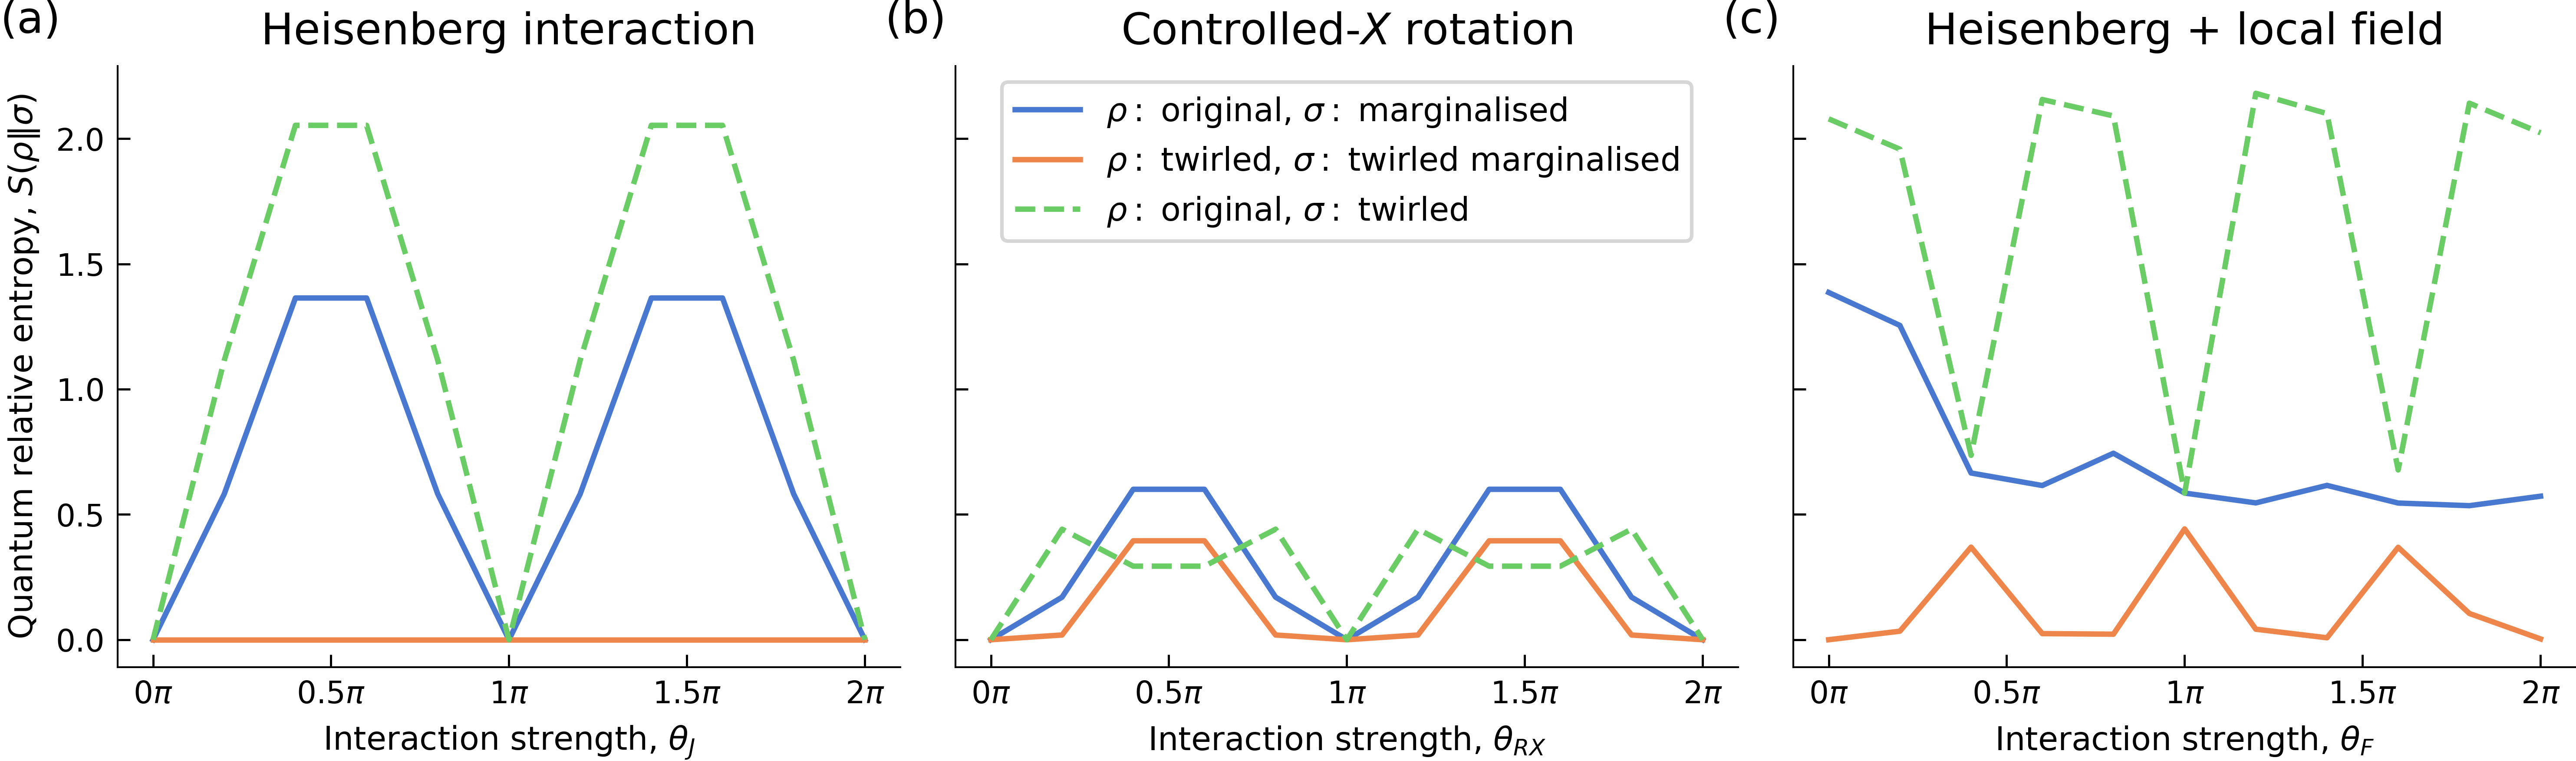
\includegraphics[width=1\textwidth]{figures/worked_examples1.pdf}
    \caption{\textbf{Quantum relative entropy diagnostics of SPPs.} We plot the generalised quantum mutual information \(\mathcal{I}[\Upsilon_{0:1}] = S(\Upsilon_{0:1} \| \Upsilon_{0:1}^{\mathrm{Markov}})\), its twirled counterpart \(\mathcal{I}[\Upsilon_{0:1}^{\mathcal{T}_P}]\), and the twirl relative entropy \(\mathcal{J}[\Upsilon_{0:1}]\) as functions of interaction strength \(\theta\in[0,2\pi]\) for three different Hamiltonian families. Choi operators are normalised such that \(\Tr[\Upsilon_{0:1}] = 1\), and the environment is initialised in \(\ket{+}\). Panels: (a) Heisenberg exchange interaction, (b) controlled-\(X\) rotation, (c) Heisenberg exchange with local field.
    }
    \label{fig:worked-examples-entropies}
\end{figure}

We evaluate \(\mathcal{I}[\Upsilon_{0:1}]\), \(\mathcal{I}[\Upsilon_{0:1}^{\mathcal{T}_P}]\), and \(\mathcal{J}[\Upsilon_{0:1}]\) for each Hamiltonian family as functions of the interaction strength, where Choi operators \(\Upsilon_{0:1}\) are normalised such that \(\Tr[\Upsilon_{0:1}] = 1\). \Cref{fig:worked-examples-entropies} plots each quantity over \(\theta \in [0,2\pi]\). For the Heisenberg model in panel~(a), \(\mathcal{I}[\Upsilon_{0:1}]\) is maximal at \(\theta_J = (2n+1)\pi/2\), \(n \in \mathbb{Z}\), corresponding to a SWAP-like operation, and minimal for \(\theta_J = n\pi\), corresponding to the identity operation. Notably, the twirled process has \(\mathcal{I}[\Upsilon_{0:1}^{\mathcal{T}_P}] = 0\) for all \(\theta_J\), that is, due to the symmetry of the interaction, the induced SPP is always temporally independent.

To visualise the Pauli sequence probabilities directly, \cref{fig:worked-examples-probabilities} plots \(\Pr(\mathcal{P}_{0:1})\) at representative parameter values for each model. For the Heisenberg interaction at \(\theta_J = (2n + 1)\pi/2\) in panel~(a), the resulting SPP is a uniform distribution over all 16 possible Pauli trajectories, corresponding to maximally depolarising noise at each step; correspondingly, \(\mathcal{J}[\Upsilon_{0:1}]\) is maximal, indicating the original process is farthest from its twirled counterpart.

For the \(H_{RX}\) model in \cref{fig:worked-examples-entropies}(b), the GQMI is non-zero for both the original and twirled processes, indicating the presence of temporal correlations in the induced SPP. In particular, at \(\theta_{RX} = \pi/2\), we find \(\mathcal{I}[\Upsilon_{0:1}] = \mathcal{I}[\Upsilon_{0:1}^{\mathcal{T}_P}] = \ln 2\) and \(\mathcal{J}[\Upsilon_{0:1}] = 0\), showing that the original process is Pauli-twirl invariant and hence already an SPP. This is reflected in the trajectory distribution in \cref{fig:worked-examples-probabilities}(b), where only the \(I_{t_0}I_{t_1}\) and \(X_{t_0}X_{t_1}\) sequences occur with non-zero probability, corresponding to a perfectly two-time correlated bit-flip channel. Away from these special points at \(\theta_{RX} \neq n\pi/2\), we observe that the twirling generally reduces the GQMI while \(\mathcal{J}[\Upsilon_{0:1}]\) increases, consistent with the removal of non-Pauli structure and non-Pauli-based temporal correlations.

Finally, for the local field model in \cref{fig:worked-examples-entropies}(c), we observe a non-trivial interplay between the exchange interaction and the symmetry-breaking local field. The GQMI \(\mathcal{I}[\Upsilon_{0:1}]\) is maximal at \(\theta_F = 0\) (pure Heisenberg dynamics) and then decays non-monotonically as the field strength increases. In contrast to the Heisenberg-only case, the twirled GQMI \(\mathcal{I}[\Upsilon_{0:1}^{\mathcal{T}_P}]\) is generically non-zero and displays oscillatory peaks and troughs as a function of \(\theta_F\). The twirl relative entropy \(\mathcal{J}[\Upsilon_{0:1}]\) exhibits two distinct types of troughs which alternate with peaks in \(\mathcal{I}[\Upsilon_{0:1}^{\mathcal{T}_P}]\). The trajectory probabilities in \cref{fig:worked-examples-probabilities}(c) are dominated by the \(I_{t_0}I_{t_1}\) sequence, with small but correlated contributions from the Pauli sequences excluding an identity. Overall, this model highlights that SPPs can exhibit rich and structured temporal correlations, even when genuinely quantum temporal correlations are discarded.

\begin{figure}
    \centering
    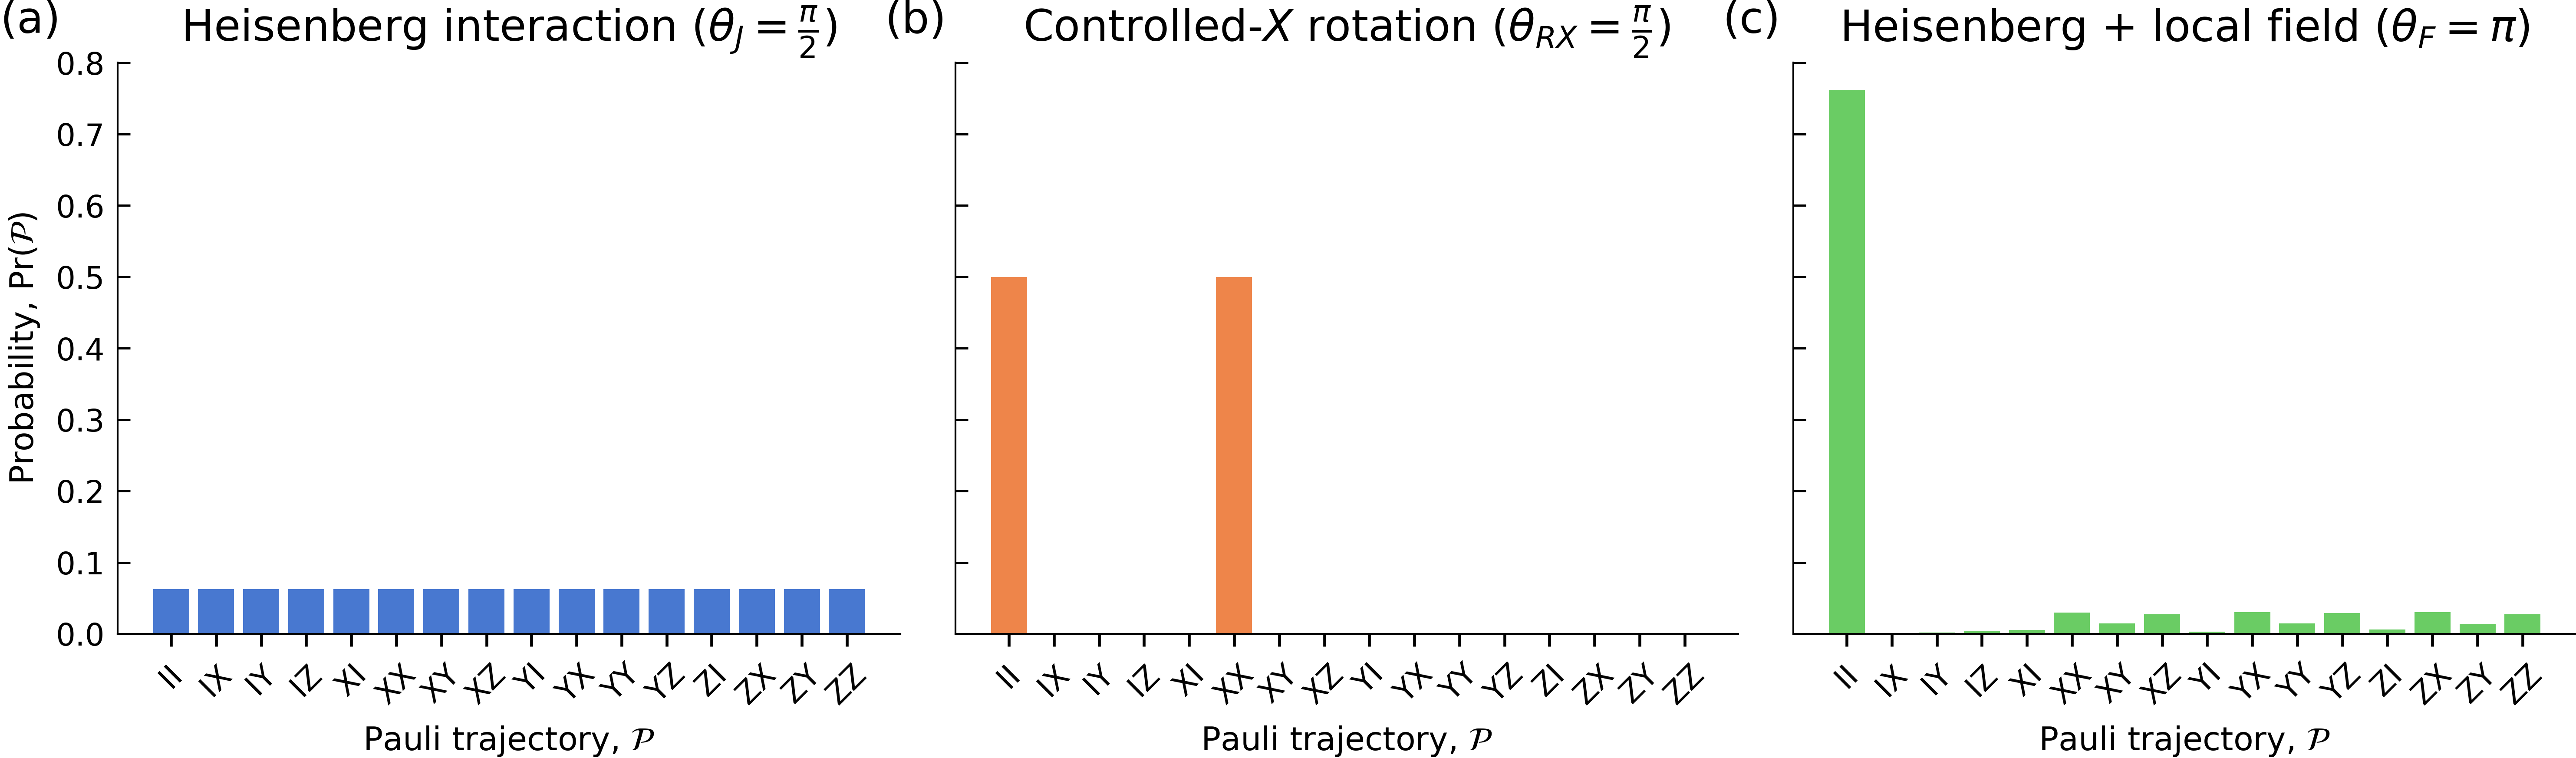
\includegraphics[width=1\textwidth]{figures/worked_examples2.pdf}
    \caption{\textbf{Example single-slot SPP trajectory distributions.} (a) Heisenberg exchange interaction for \(\theta_J = \pi/2\), (b) controlled-\(X\) rotation for \(\theta_{RX} = \pi/2\), (c) Heisenberg exchange with local field for \(\theta_F = \pi\).}
    \label{fig:worked-examples-probabilities}
\end{figure}

Having established the SPP framework and illustrated it with worked examples, we now analyse temporal correlations in one-dimensional SPP MPS representations, developing a transfer operator framework to characterise memory and correlation decay.
